\section*{Appendix}
\subsection*{Comparison with Other MBRL Methods}
% use figure
\begin{figure}[htbp]
  \centering
  \begin{subfigure}[b]{0.33\columnwidth}
    \centering
    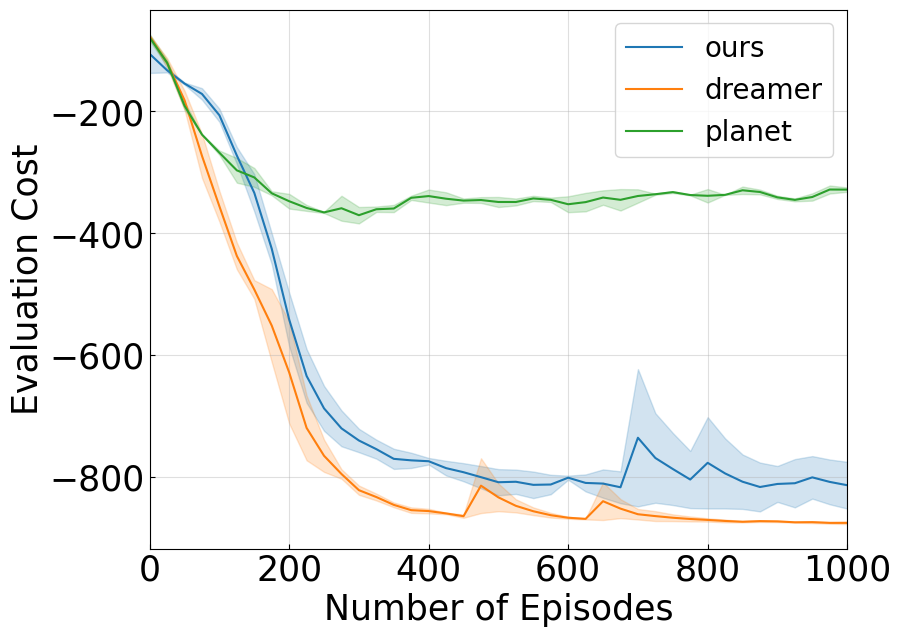
\includegraphics[width=\columnwidth]{figures/comp_mbrl_sm06_cartpole_pixel.png}
    \caption{Cart-Pole with Pixel Observation}
    \label{fig:comp_mbrl_cartpole_pixel}
  \end{subfigure}%
  \hfill
  \begin{subfigure}[b]{0.33\columnwidth}
    \centering
    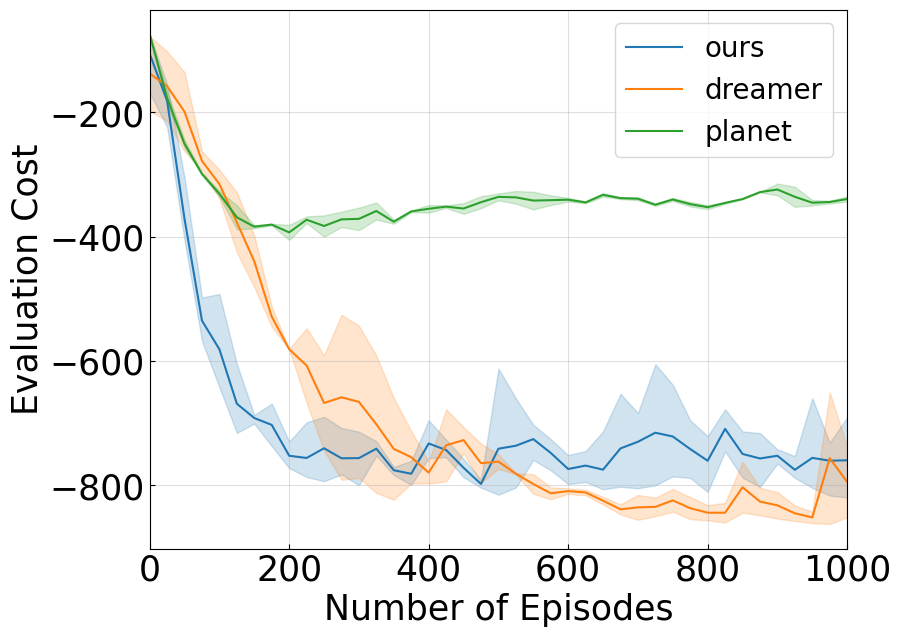
\includegraphics[width=\columnwidth]{figures/comp_mbrl_sm06_cartpole_fc.png}
    \caption{Cart-Pole with 4D state}
    \label{fig:comp_mbrl_cartpole_fc}
  \end{subfigure}%
  \hfill
    \begin{subfigure}[b]{0.33\columnwidth}
    \centering
    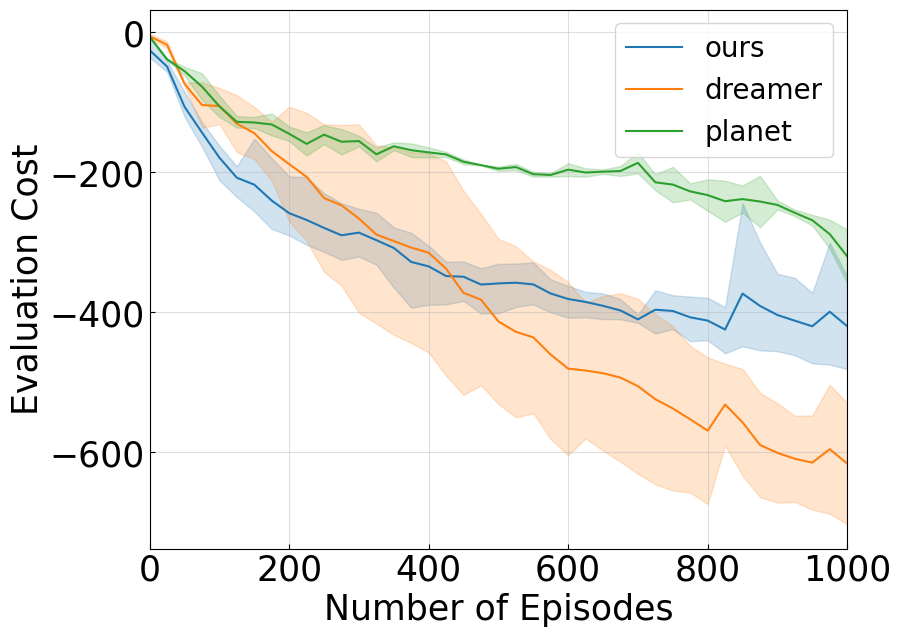
\includegraphics[width=\columnwidth]{figures/comp_mbrl_sm06_cheetah.png}
    \caption{Cheetah Running with 18D state}
    \label{fig:comp_mbrl_cheetah}
  \end{subfigure}%
  \caption{Comparison with well-known model-based RL methods.}
  \label{fig:three_images_comp_mbrl}
\end{figure}
To benchmark our approach against established model-based RL methods, we select two widely recognized methods: PlaNet \cite{hafner2019learning} and Dreamer (Version 2) \cite{hafner2020mastering}. This comparison spans three tasks in the main paper. Remarkably, across all three tasks, our method demonstrates a clear superiority over PlaNet in terms of both data efficiency and peak performance. Additionally, our method achieves competitive performance with Dreamer-v2 in two Cart-Pole experiments, along with comparable data efficiency in cheetah running tasks. It's important to note that this comparable performance is achieved while our method learns a globally linear model, whereas Dreamer employs a much larger nonlinear network to approximate a world model. Therefore, our approach achieves a substantial reduction in both computational demands and structural complexity while not compromising control performance too much. It is also worth noting that our approach stands out from commonly used Model-Based RL methods as it's rooted in Koopman theory, offering the advantage of enabling control theory analysis for the system.

\subsection*{Comparison with Other Encoders and Losses}
\begin{figure}[htbp]
  \centering
  \begin{subfigure}[b]{0.33\columnwidth}
    \centering
    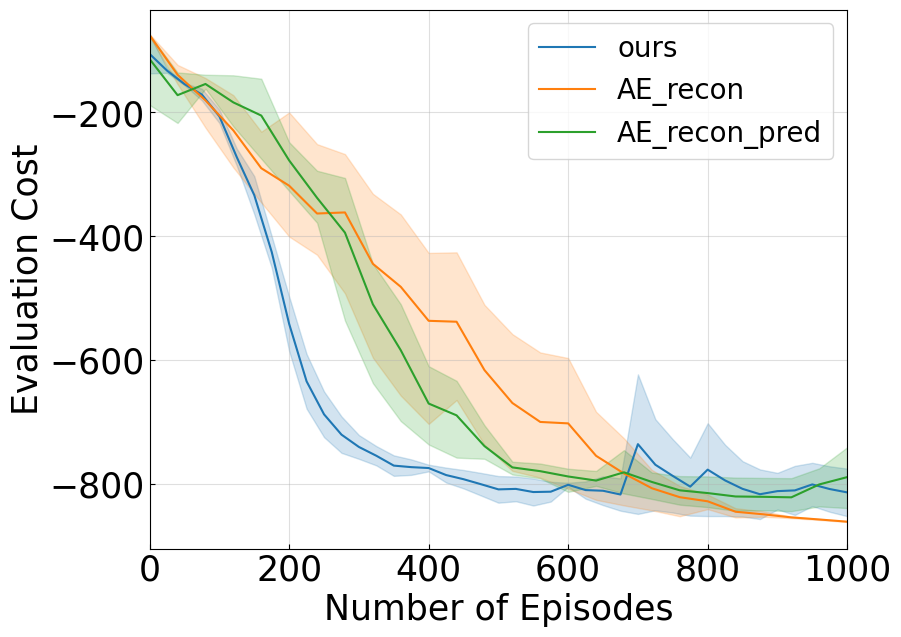
\includegraphics[width=\columnwidth]{figures/comp_ae_sm06_cartpole_pixel_new.png}
    \caption{Cart-Pole with Pixel Observation}
    \label{fig:comp_ae_cartpole_pixel}
  \end{subfigure}%
  \hfill
  \begin{subfigure}[b]{0.33\columnwidth}
    \centering
    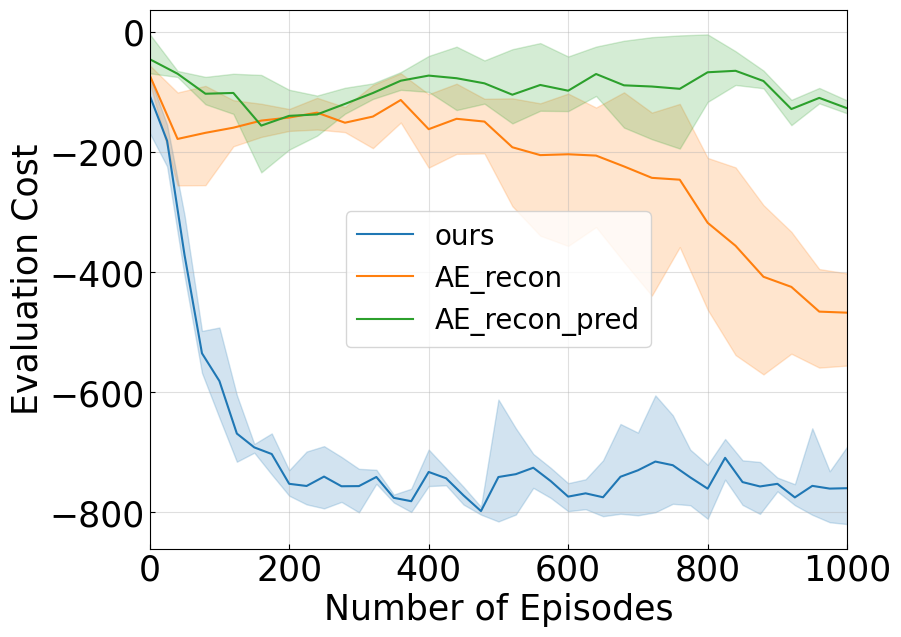
\includegraphics[width=\columnwidth]{figures/comp_ae_sm06_cartpole_fc_new.png}
    \caption{Cart-Pole with 4D state}
    \label{fig:comp_ae_cartpole_fc}
  \end{subfigure}%
  \hfill
    \begin{subfigure}[b]{0.33\columnwidth}
    \centering
    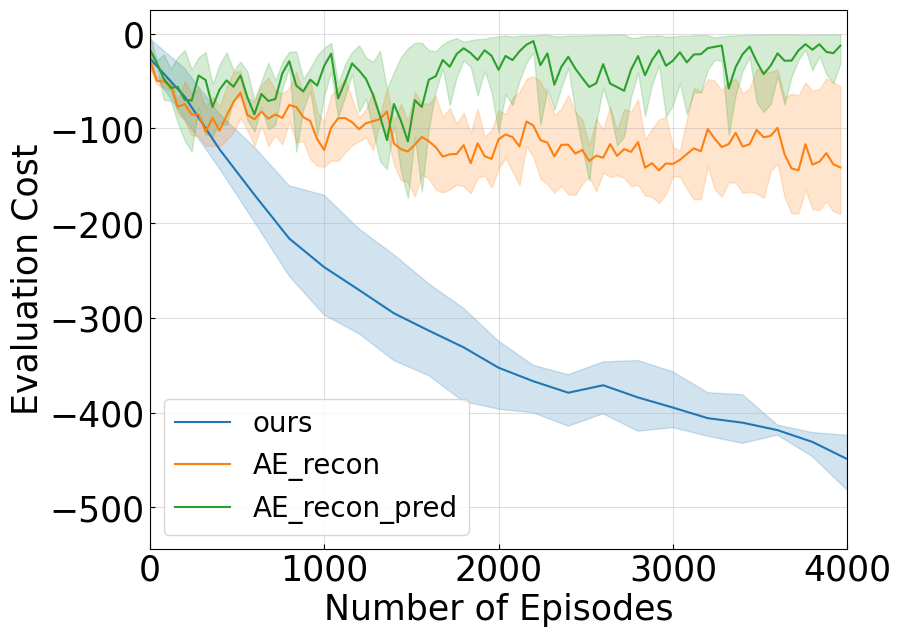
\includegraphics[width=\columnwidth]{figures/comp_ae_sm06_cheetah_new.png}
    \caption{Cheetah Running with 18D state}
    \label{fig:comp_ae_cheetah}
  \end{subfigure}%
  \caption{Comparison with autoencoder and varying losses.}
  \label{fig:three_images_comp_ae}
\end{figure}


We perform experiments to validate our selection of the contrastive embedding function. To achieve this, we replace the contrastive encoder with a canonical autoencoder (AE), a commonly used method for learning condensed representations from high-dimensional observations. Specifically, we utilize the AE along with two types of loss functions: one involving only reconstruction loss, and another involving a combination of reconstruction and one-step prediction loss. Importantly, we keep all other aspects of our method unchanged. Results are based on 3 random seeds.

As shown in Figure.~\ref{fig:three_images_comp_ae}, our approach achieves comparable control performance with the use of AE. This aligns with the notion that autoencoder excels in reconstructing and representing pixel-based observations. However, when tasks involve non-pixel observations, such as normal states, our approach still maintains significant control efficiency and performance, while the AE-based structure struggles to learn a useful policy even with ample data. Particularly, we observed that the AE with only reconstruction loss slightly outperforms the one employing the combined loss, but still falls short of achieving the performance obtained by our method using the contrastive encoder. These results provide validation for our choice of contrastive embedding function within our approach.

\subsection*{Ablations Study of Hyper-parameters}
We undertook an ablation study involving key parameters of the LQR solving iteration and Koopman embedding dimension. Results are the mean over 3 random seeds and summarized in  Table.~\ref{tab:my-table}.

We found that our approach remains robust regardless of the specific number of iterations used for the LQR solution, as long as it falls within a reasonable range. This suggests that achieving a certain level of precision in solving the Riccati Equation contributes positively to both policy and linear model learning. We also studied the impact of varying the latent embedding dimensions for the encoder. Our findings indicate that using a smaller dimension that aligns with the encoder's intermediate layers yields consistently good results, while excessively increasing the embedding dimension (d=100) can diminish control performance. One reason could be the reduced approximation capabilities of the encoder due to inappropriate high latent dimension. It might also be because the latent state becoming overly sparse 
and failing to capture crucial information for effective control.

\begin{table}[!htp]
\scriptsize
\centering
\resizebox{\columnwidth}{!}{%
\begin{tabular}{|cc|ccc|ccc|}
\hline
\multicolumn{2}{|c|}{\multirow{2}{*}{}} &
  \multicolumn{3}{c|}{LQR iteration} &
  \multicolumn{3}{c|}{Latent Dimension} \\ \cline{3-8} 
\multicolumn{2}{|c|}{} &
  \multicolumn{1}{c|}{iter=3} &
  \multicolumn{1}{c|}{iter=5*} &
  iter=10 &
  \multicolumn{1}{c|}{d=30} &
  \multicolumn{1}{c|}{d=50*} &
  d=100 \\ \hline
\multicolumn{1}{|c|}{\multirow{2}{*}{cartpole pixel}} &
  control cost  &
  \multicolumn{1}{c|}{-863} &
  \multicolumn{1}{c|}{-873} &
  -835 &
  \multicolumn{1}{c|}{-848} &
  \multicolumn{1}{c|}{-873} &
  -813 \\ \cline{2-8} 
\multicolumn{1}{|c|}{} &
  model error  &
  \multicolumn{1}{c|}{0.075} &
  \multicolumn{1}{c|}{0.058} &
  0.269 &
  \multicolumn{1}{c|}{0.165} &
  \multicolumn{1}{c|}{0.058} &
  0.038 \\ \hline
\multicolumn{1}{|c|}{\multirow{2}{*}{cartpole state}} &
  control cost  &
  \multicolumn{1}{c|}{-751} &
  \multicolumn{1}{c|}{-762} &
  -769 &
  \multicolumn{1}{c|}{-777} &
  \multicolumn{1}{c|}{-762} &
  -667 \\ \cline{2-8} 
\multicolumn{1}{|c|}{} &
  model error  &
  \multicolumn{1}{c|}{0.00047} &
  \multicolumn{1}{c|}{0.00031} &
  0.00042 &
  \multicolumn{1}{c|}{0.00043} &
  \multicolumn{1}{c|}{0.00031} &
  0.0002 \\ \hline
\multicolumn{1}{|c|}{\multirow{2}{*}{cheetah run}} &
  control cost  &
  \multicolumn{1}{c|}{-436} &
  \multicolumn{1}{c|}{-464} &
  -448 &
  \multicolumn{1}{c|}{-477} &
  \multicolumn{1}{c|}{-464} &
  -235 \\ \cline{2-8} 
\multicolumn{1}{|c|}{} &
  model error  &
  \multicolumn{1}{c|}{0.732} &
  \multicolumn{1}{c|}{0.862} &
  0.842 &
  \multicolumn{1}{c|}{0.653} &
  \multicolumn{1}{c|}{0.862} &
  0.046 \\ \hline
\end{tabular}%
}
\caption{\small Ablation results of final cost and model-fitting error regarding LQR solving iteration and Koopman latent state dimension. The asterisk refers to the parameter used in the main paper.}
\label{tab:my-table}
\end{table}

% \subsection*{Real-World Evaluation}
% In this real robot task, we deploy our algorithm trained from the Gazebo simulator to the turtlebot3 burger ground robot. We use 2D Lidar measurements as well as the odometry information as observation, and the linear LQR policy generates the linear and angular velocities as control. We aim to control the robot to navigate through a narrow curved path without any collisions. We directly transfer the trained policy (which is trained with only 40 episodes and each episode contains around 700 steps) to the hardware without any fine-tuning, indicating the applicability of our approach to a real robot.

% \begin{figure}[htbp]
%   \centering
%   \begin{subfigure}[b]{0.13\columnwidth}
%     \centering
%     \includegraphics[width=\columnwidth]{figures/real_experiement_curve_navigation - frame at 0m4s.jpg}
%     \caption{4s}
%     \label{fig:real_a}
%   \end{subfigure}%
%   \hfill
%   \begin{subfigure}[b]{0.13\columnwidth}
%     \centering
%     \includegraphics[width=\columnwidth]{figures/real_experiement_curve_navigation - frame at 0m9s.jpg}
%     \caption{9s}
%     \label{fig:real_b}
%   \end{subfigure}%
%   \hfill
%   \begin{subfigure}[b]{0.13\columnwidth}
%     \centering
%     \includegraphics[width=\columnwidth]{figures/real_experiement_curve_navigation - frame at 0m15s.jpg}
%     \caption{15s}
%     \label{fig:real_c}
%   \end{subfigure}%
%   \begin{subfigure}[b]{0.13\columnwidth}
%     \centering
%     \includegraphics[width=\columnwidth]{figures/real_experiement_curve_navigation - frame at 0m20s.jpg}
%     \caption{20s}
%     \label{fig:real_d}
%   \end{subfigure}%
%   \begin{subfigure}[b]{0.13\columnwidth}
%     \centering
%     \includegraphics[width=\columnwidth]{figures/real_experiement_curve_navigation - frame at 0m26s.jpg}
%     \caption{26s}
%     \label{fig:real_e}
%   \end{subfigure}%
%   \begin{subfigure}[b]{0.13\columnwidth}
%     \centering
%     \includegraphics[width=\columnwidth]{figures/real_experiement_curve_navigation - frame at 0m29s.jpg}
%     \caption{29s}
%     \label{fig:real_f}
%   \end{subfigure}%
%   \begin{subfigure}[b]{0.13\columnwidth}
%     \centering
%     \includegraphics[width=\columnwidth]{figures/real_experiement_curve_navigation - frame at 0m30s.jpg}
%     \caption{30s}
%     \label{fig:real_g}
%   \end{subfigure}%
%   \caption{Snapshots of real robot curved trajectory at different time stamps (seconds).}
%   \label{fig:real}
% \end{figure}

\textbf{Interpretable Q Matrix in Latent Space.}

\begin{wrapfigure}{r}{0.4\columnwidth}
\vspace{-25pt}
  \centering
  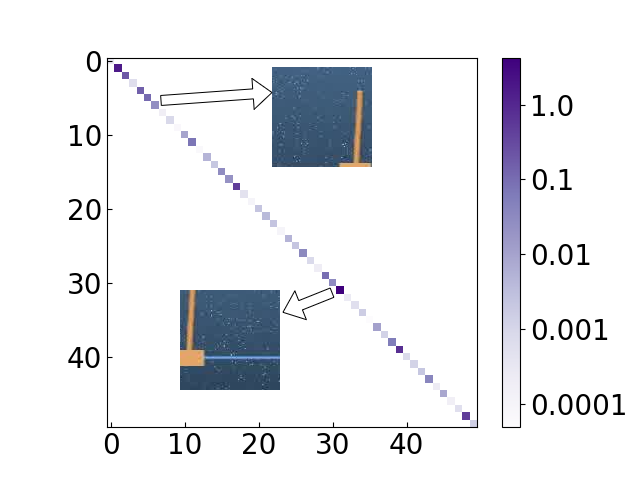
\includegraphics[width=0.4\columnwidth]{figures/ituitiveQ.png}
  \caption{\small Relations of learned weights in latent $\mathbf{Q}$ matrix and original pixel states}
  \label{fig:interpretable_Q}
\end{wrapfigure}
One key distinction of our method from CURL \cite{laskin2020curl} is the utilization of a structured LQR policy in the latent space. In Fig.~\ref{fig:interpretable_Q}, we illustrate that the LQR policy parameters, especially the Q matrix, can capture the relative significance weights of latent embedding and their relationship to the original pixel states. We take the pixel-based CartPole task as an example. The larger diagonal elements in the learned Q matrix correspond to visual patches that contain the CartPole object, which provides interpretable information that captures useful latent information related to the CartPole object's area in the image 